\documentclass[11pt, a4paper]{MATH2023}
\usepackage{fancyhdr}
\usepackage{setspace}
\usepackage{amsmath,mathrsfs}
\usepackage{multicol}
\usepackage{amssymb}
\usepackage{graphicx}
\usepackage{caption}
\usepackage{subcaption}
\usepackage{xcolor}
\usepackage{enumitem}
\usepackage{tikz}
\usepackage{mathtools}
\usetikzlibrary{matrix}
\usepackage[normalem]{ulem}
\usepackage{multirow}
\usepackage[linesnumbered, ruled, boxed]{algorithm2e}
\SetKwRepeat{Do}{do}{while}
\newcommand{\eg}{\textbf{[Example.] }}
\newcommand{\sol}{\textbf{[Solution.] }}
\newcommand{\ii}{{\bf i}}
\newcommand{\jj}{{\bf j}}
\newcommand{\kk}{{\bf k}}
\newcommand{\rr}{{\bf r}}
\newcommand{\FF}{{\bf F}}
\renewcommand{\div}{{\rm div\ }}
\newcommand{\curl}{{\rm curl\ }}
\newcommand{\pt}{\partial}


\title{Chapter 13}
\subtitle{Application of Partial Derivatives}

\begin{document}
\begin{spacing}{1.3}

    \section{Extreme Values}
    {\blue Recall that in single variable calculus:

    $x_1$ is a {\it relative} maximum point, if $f'(x_1)=0$ and $f''(x_1)<0$,\\
    $x_2$ is a {\it relative} minimum point, if $f'(x_2)=0$ and $f''(x_2)>0$.
    }

    Similarly, in multi-variable calculus, the {\bf critical point} is where 
    \begin{center}
        \boxed{$$\disp \nabla f(\rr_0)=(f_{x_1}(\rr_0), f_{x_2}(\rr_0),\cdots,f_{x_n}(\rr_0))={\bf 0}$$}
    \end{center}
    

    And, if $h$ has a {\bf relative extremum} at a point $\rr_0$, then $\rr_0$ is a {\bf critical point},
    and $\nabla f(\rr_0)={\bf 0}$.
    However, if $\rr_0$ is a critical point, we {\it cannot infer} that $\rr_0$ is a relative extremum.
    The reason is similar in single variable calculus.

    \vspace{0.4in}
    Different from single variable, a critical point which {\it is not a relative extremum} is a {\bf saddle point}.
    \begin{center}
        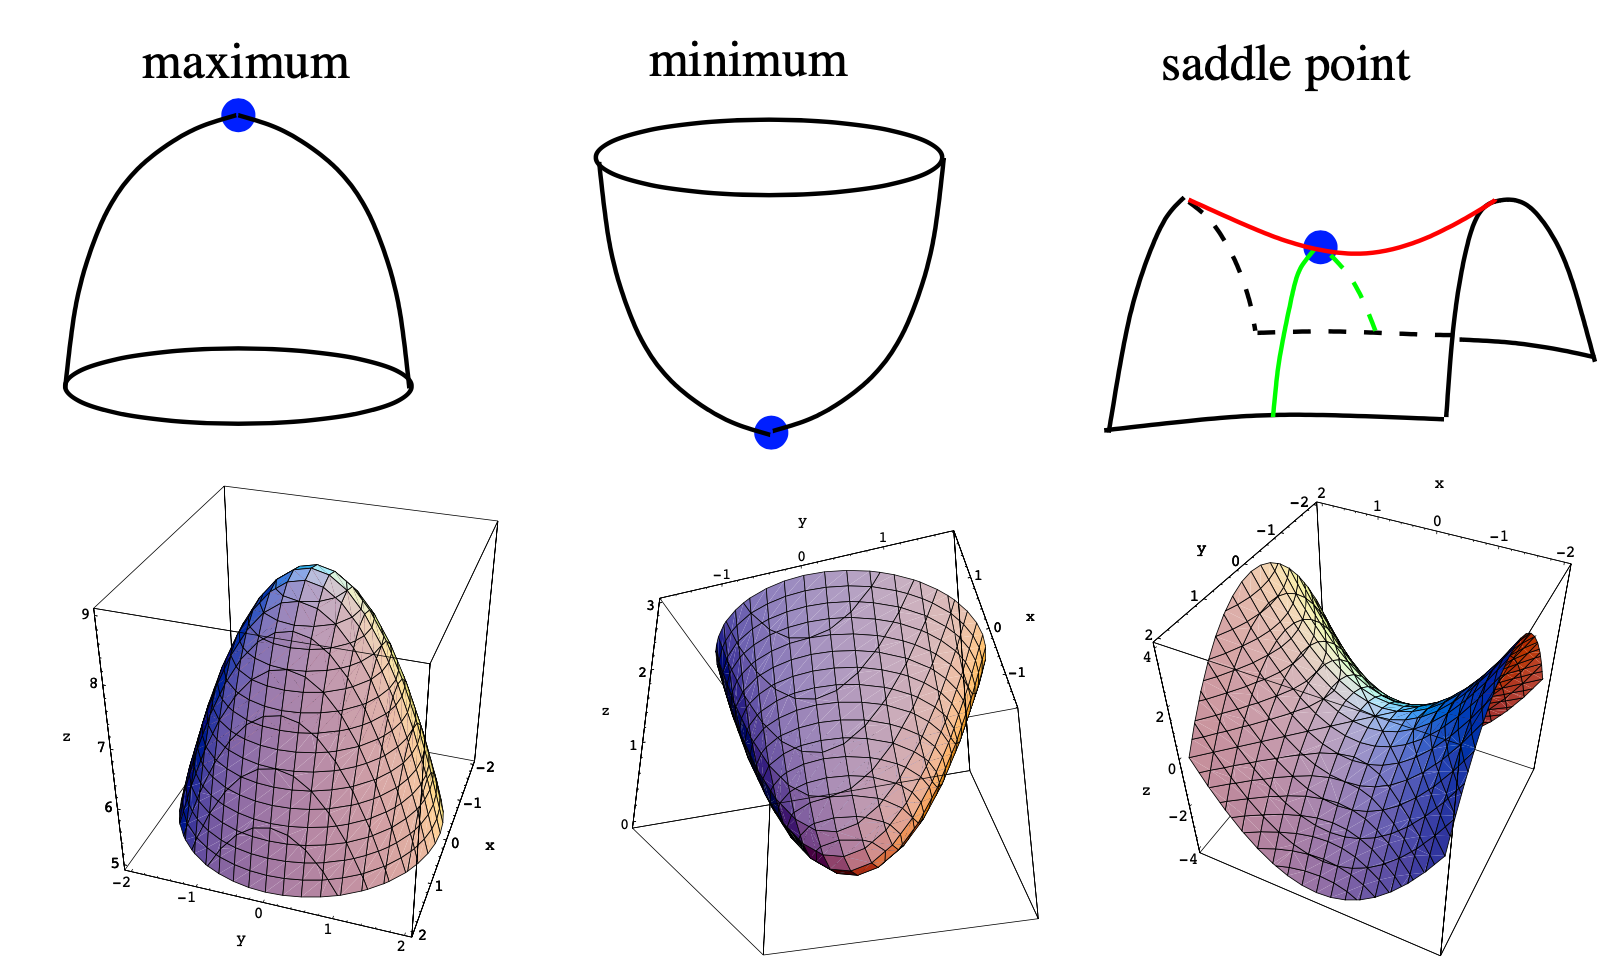
\includegraphics[scale=0.4]{images/Ch13-saddle.png}
    \end{center}

    \newpage
    However, to classify the critical points, we need the {\bf second derivative test}, or {\bf D-test}.

    \vspace{0.3in}
    {\bf Second Derivative Test}

    Suppose $f(x, y)$ has a critical point at $\mathbf{r}_{0}=\left(x_{0}, y_{0}\right)$ 
    (i.e. $\left.\nabla f\left(\mathbf{r}_{0}\right)=\mathbf{0}\right)$ and the second partial 
    derivative of $f(x, y)$ are continuous in a disk with center $\mathbf{r}_{0}=\left(x_{0}, y_{0}\right) .$ Let
    \begin{center}
        \boxed{$$\disp 
        D=\left|\begin{array}{ll}
        f_{x x}\left(\mathbf{r}_{0}\right) & f_{x y}\left(\mathbf{r}_{0}\right) \\
        f_{y x}\left(\mathbf{r}_{0}\right) & f_{y y}\left(\mathbf{r}_{0}\right)
        \end{array}\right|=f_{x x}\left(\mathbf{r}_{0}\right) f_{y y}\left(\mathbf{r}_{0}\right)-f_{x y}^{2}\left(\mathbf{r}_{0}\right)
        $$}
    \end{center}
    
    \begin{center}
        \begin{tabular}{c|c|c}
            \hline\hline 
            $D$ & $f_{x x}\left(\mathbf{r}_{0}\right)$ or $f_{y y}\left(\mathbf{r}_{0}\right)$ & nature of $\mathbf{r}_{0}$ \\\hline\hline
            $>0$ & $>0$ & relative minimum \\\hline
            $>0$ & $<0$ & relative maximum \\\hline
            $<0$ & & saddle point \\\hline
            $=0$ & & no conclusion can be drawn \\\hline
        \end{tabular}
    \end{center}
    
    \vspace{0.4in}
    {\it I'd like to omit the proof of D-Test here.}

    \vspace{0.8in}
    {\blue This example shows basic use of D-Test.}

    \eg Find the relative minima and maxima of $f(x, y)=x^{3}+y^{3}-3 x-12 y+20$.
    $$
    f_{x}=3 x^{2}-3 \quad \text { and } \quad f_{y}=3 y^{2}-12
    $$

    \sol 
    For critical points, $f_{x}=f_{y}=0 \quad \Rightarrow \quad x=\pm 1, y=\pm 2$.

    $\therefore (1,2),(-1,2),(1,-2),(-1,-2)$ are critical points.

    To apply D-Test, compute:
    $f_{xx}=6x, f_{yy}=6y, f_{xy}=0$, hence $D=f_{xx}\cdot f_{yy}-(f_{xy})^2= 36xy$

    \begin{center}
        \begin{tabular}{c|c|c|c|c|c}\hline\hline
            Point & $f_{xx}$ & $f_{yy}$ & $f_{xy}$ & $D$ & Type\\\hline\hline
            $(1,2)$ & 6 & 12 & 0 & 72 & min \\\hline
            $(-1,2)$ & $-6$ & 12 & 0 & $-72$ & saddle\\\hline
            $(1,-2)$ & 6 & $-12$ & 0 & $-72$ & saddle\\\hline
            $(-1,-2)$ & $-6$ & $-12$ & 0 & 72 & max\\\hline
        \end{tabular}
    \end{center}



    \newpage
    {\blue This example shows how to find extrema on a {\it closed} and {\it bounded} region.}

    \eg Find the absolute extrema of the function
    $$z=f(x, y)=x y-x-3 y$$
    on the {\it closed} and {\it bounded} set $R$, where $R$ is the triangular 
    region with vertices $(0,0),(0,4)$ and $(5,0)$.

    \sol $f_x=y-1, f_y=x-3, f_{xy}=f_{yx}=1, f_{xx}=f_{yy}=0, D=-1$

    For critical points, $\nabla f=(f_x, f_y)=(0,0) \Rightarrow x=3, y=1$.

    This point is inside the domain. But we still need to find possible 
    extreme points {\it on the boundary of domain}.

    {\bf (1)} Along $OA:$, $\rr_0=(0,0), \rr_1=(5,0)$, so the parametric representation 
    of line $OA$ is:
    $$\rr(t)=(1-t)\rr_0+t\rr_1,=(5t, 0),\ t\in [0,1]$$
    hence $z=f(\rr(t))=-5t,\ t\in [0,1]$

    So along $OA$, the possible extreme points are $(0,0)$ and $(5,0)$.

    {\bf (2)} Along $OB:$, similarly, $\rr(t)=(0, 4t),\ t\in [0,1]$, 
    $z=f(\rr)=-12t$,

    So along $OB$, the possible extreme points are $(0,0)$ and $(0,4)$.

    {\bf (3)} Along $AB:$ $\rr(t)=(5-5t, 4t),\ t\in [0,1]$,
    $z=-20t^2+13t-5,\ t\in [0,1]$

    There is one critical point on $AB$, when $dz/dx=0$, at $\left(\dfrac{27}{8}, \dfrac{13}{10}\right)$.

    Then we compute the value of all possible extremum points,
    \begin{center}
        \begin{tabular}{c|c}\hline\hline
            $(x,y)$ & $f(x,y)$ \\\hline\hline
            $(3,1)$ & $-3$\\\hline
            $\left(\dfrac{27}{8}, \dfrac{13}{10}\right)$ & $-\dfrac{231}{80}$\\\hline
            $(0,0)$ & 0 \\\hline
            $(5,0)$ & $-5$ \\\hline
            $(0,4)$ & $-12$ \\\hline
        \end{tabular}
    \end{center}

    Therefore, absolute maximum value is 0 which occurs at $(0,0)$,
    absolute minimum value is $-12$ which occurs at $(0,4)$. 


    \vspace{0.2in}
    {\blue This example converts the problem to max/min problem.}

    \eg Find the points on the surface $z^2=xy+1$ that are closest to the origin.

    \sol $d^2=(x-0)^2+(y-0)^2=x^2+y^2+xy+1=f(x,y)$, only need to minimize this function.


    \newpage
    {\blue This is a more comprehensive and tricker problem.}

    \eg Find absolute minimum and maximum value of $f(x,y)=2x^3+y^4$ on the set 
    $D=\{(x,y)|x^2+y^2\le 1\}$.

    \sol First, find the critical point of $f(x,y)$ on entire $xy$ plane.

    $f_x=6x^2, f_y=4y^3$, critical points: $f_x=f_y=0\Rightarrow x=y=0$, and $f(0,0)=0$.

    Then, on the circle $x^2+y^2=1$, eliminate $y$, we have:
    \begin{align*}
        g(x) &= f(x,y)=x^4+2x^3-2x^2+1,\ -1\le x\le 1\\
        g'(x) &= 4x^3+6x-4x=0
    \end{align*}
    the equation has solutions: $(x,y)=(0, \pm 1), \left(\frac{1}{2}, \frac{\sqrt{3}}{2}\right)$,
    to check each of them:
    $$f(0, \pm 1)=g(0)=1,\ f\left(\frac{1}{2}, \frac{\sqrt{3}}{2}\right)=g\left(\frac{1}{2}\right)=\frac{13}{16}$$
    Also, we need to check the {\it endpoints}, (since we are looking for min/max point of $g(x)$ on $x\in [-1,1]$)
    $$g(1)=2,\ g(-1)=-2$$
    Therefore, the absolute minimum is $g(-1)=f(-1,0)=-2$, the absolute maximum is $g(1)=f(1,0)=2$.

    \vspace{0.5in}
    Notice that, if you are interested in the nature of the critical point at $(0,0)$, you may try $D$-test:
    $$D=f_{xx}f_{yy}-f_{xy}^2=144xy^2=0\ \text{\ ,\ at (0,0)}$$
    so the $D$-test fails, we have to use other methods to determine it:

    In the plane $y=0$, $f(x,0)=2x^3$, and in the plane $x=0$, $f(0,y)=y^4$.
    \begin{center}
        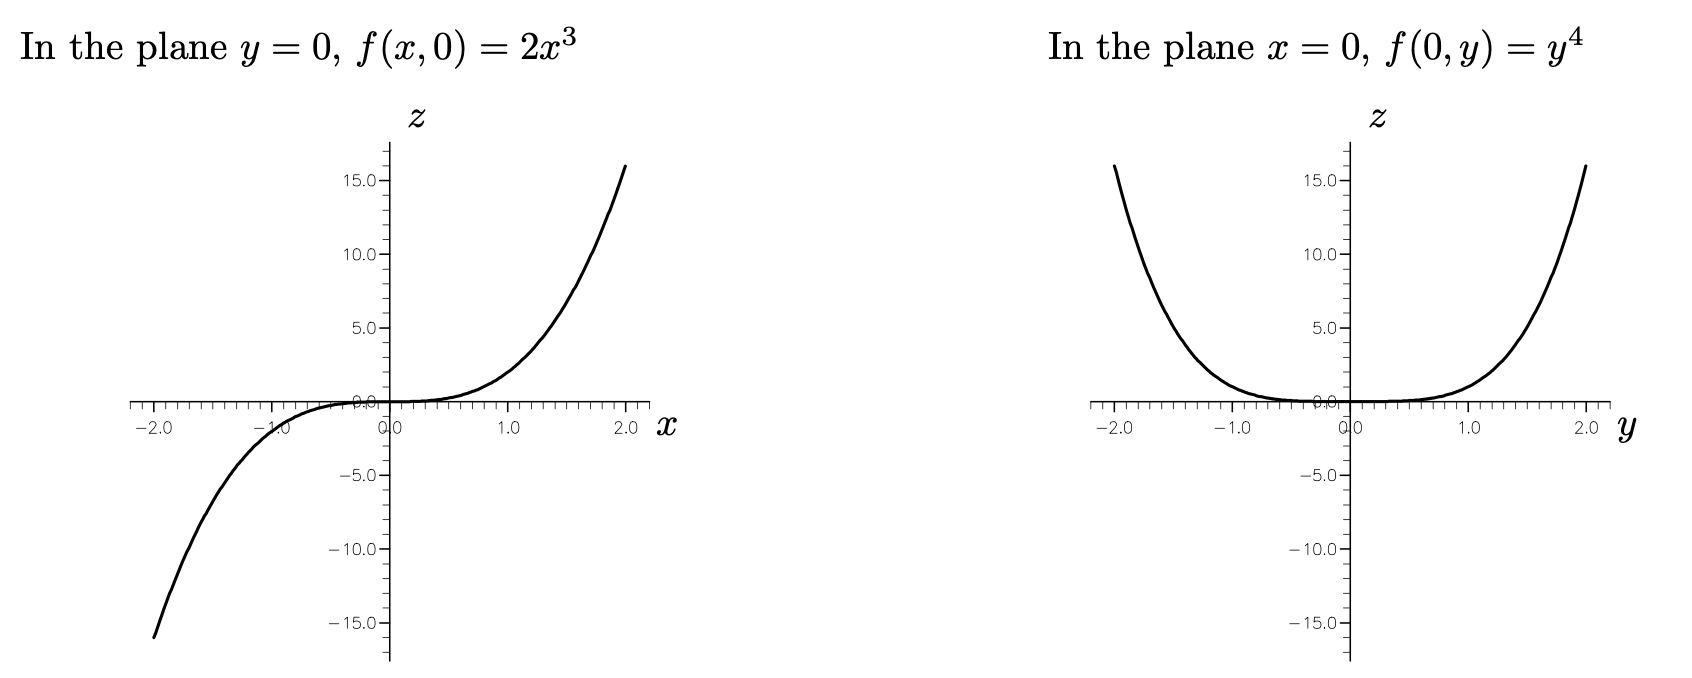
\includegraphics[scale=0.46]{images/Ch13-ex1.4.png}
    \end{center}
    Thus, the critical point is a {\it saddle point.}


    \newpage
    \section{Lagrange multipliers}

    {\blue Motivation: sometimes we want to maximize/minimize $f(x,y)$ subject to $g(x,y)=k$.}

    {\bf How to find the maximum or minimum value?}
    \begin{enumerate}
        \item Find all values of $\mathbf{r}$ and $\lambda$ such that
        $$\nabla f(\mathbf{r})=\lambda \nabla g(\mathbf{r})$$
        and $$g(\mathbf{r})=k$$
        \item Evaluate $f$ at all the points $\mathbf{r}$ that arise from step (1). 
        The largest (smallest) of these values is the maximum (min) value of $f$.
    \end{enumerate}

    {\it \textbf{Remark:}} Lagrange's method only finds critical points, 
    it {\it does not tell} whether the function is maximized or minimized.

    \vspace{0.5in}
    {\bf Proof of Lagrange's method:}

    Notice that, maximizing or minimizing a function $f(x_1,x_2,\cdots,x_n)$
    subject to a constraint of $g(x_1,x_2,\cdots,x_n)=k$ is to restrict 
    the point $(x_1,x_2,\cdots,x_n)$ to lie on the {\it level surface} $S$
    given by $g(x_1,x_2,\cdots,x_n)=k$. For example, if $n=2$, 
    maximize(or minimize) $z=f(x,y)$ subject to constraint curve $C:g(x,y)=k$
    (shown in {\green green}) is to restrict the point $(x,y)$ to lie on the {\red red} curve.
    \begin{center}
        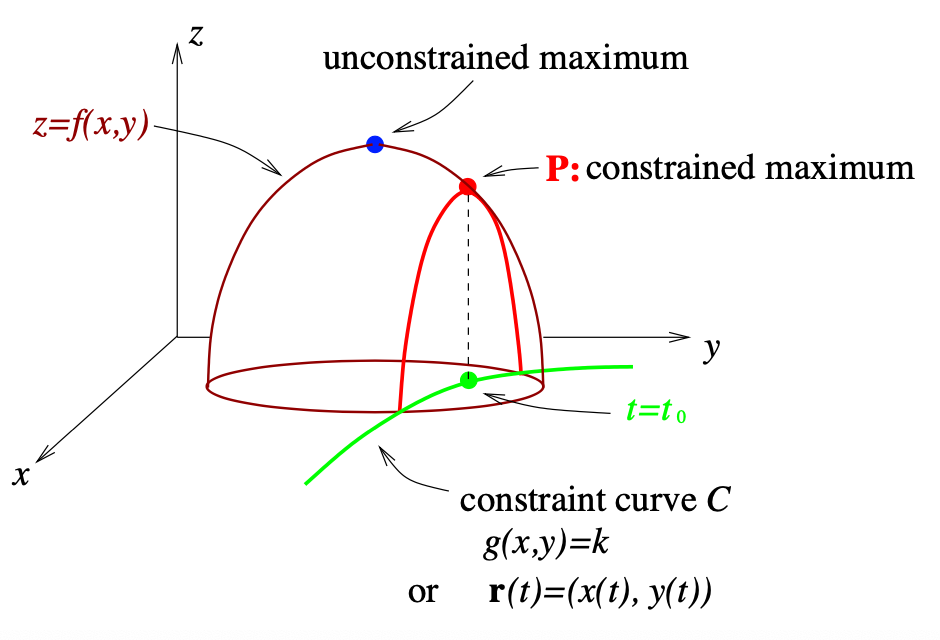
\includegraphics[scale=0.45]{images/Ch13-lag-proof.png}
    \end{center}
    Suppose $z$ has a maximum value at a point $\mathbf{P}$, and let $C$ be the {\it constraint curve} 
    with vector equation
    $$\mathbf{r}(t)=x(t) \mathbf{i}+y(t) \mathbf{j} \quad \text { be on } \quad g(x, y)=k \text {. }$$
    Assume also that at the point $\mathbf{P}, t=t_{0}$. 
    
    Since on the constraint curve $C: z(t)=f(x(t), y(t))$,

    and the point $\bf P$ should be a critical point. By using the chain rule,
    $$\begin{aligned}
    \frac{d z}{d t} &=\frac{\partial f}{\partial x} \frac{d x}{d t}+\frac{\partial f}{\partial y} \frac{d y}{d t} \\
    &=\left(\frac{\partial f}{\partial x}, \frac{\partial f}{\partial y}\right) \cdot\left(\frac{d x}{d t}, \frac{d y}{d t}\right) \\
    &=\nabla f \cdot \mathbf{r}^{\prime}(t)
    \end{aligned}$$
    Then at the point $\mathbf{P}$,
    $$\left.\frac{d z}{d t}\right|_{t=t_{0}}=\nabla f\left(x\left(t_{0}\right), y\left(t_{0}\right)\right) 
    \cdot \mathbf{r}^{\prime}\left(t_{0}\right)=0 \quad \text { (since {\bf P} is critical point) }$$

    Therefore, 
    $$\nabla f\left(x\left(t_{0}\right), y\left(t_{0}\right)\right)  \perp \mathbf{r}^{\prime}\left(t_{0}\right)$$
    
    Moreover, since $\nabla g$ is normal vector to the level set,
    $$\nabla g\left(x\left(t_{0}\right), y\left(t_{0}\right)\right)  \perp \mathbf{r}^{\prime}\left(t_{0}\right) $$
    Therefore, $\nabla f \parallel \nabla g$, $\nabla f=\lambda \nabla g$.
    
    The number $\lambda$ is called a Lagrange multiplier.

    \vspace{0.5in}
    {\blue This example shows how to use Lagrange's Method.}

    \eg Find the extreme values of $f(x, y)=x^{2}-y^{2}$ subject to $x^{2}+y^{2}=1$.
    
    \sol Find $x, y$ and $\lambda$ such that
    $\nabla f=\lambda \nabla g$, where $g=x^{2}+y^{2}=1$(constant) 
    $$2 x \mathbf{i}-2 y \mathbf{j}=\lambda(2 x \mathbf{i}+2 y \mathbf{j})$$
    , which gives
    $$
    \left\{\begin{array}{rl}
        2x= & \lambda \cdot 2x\\
        -2y= & \lambda \cdot 2y
    \end{array} \right.  \qquad \Rightarrow \qquad 
    \left\{\begin{array}{lcl}
        \lambda = 1 & {\rm or} & x=0\\
        \lambda = -1 & {\rm or} & y=0\\
    \end{array} \right.
    $$
    From $x^2+y^2=1$, we have:
    \begin{align*}
        &x=0,\ y=\pm 1,\ \lambda = -1\\
        &y=0,\ x=\pm 1,\ \lambda = 1
    \end{align*}
    Therefore, $f$ has possible extreme values at point $(0,1),(0,-1),(-1,0)$ and $(1,0)$. Evaluating $f$ at these four points, we find that
    $$\begin{aligned}
        &f(0,1)=f(0,-1)=-1 \quad(\min ) \\
        &f(1,0)=f(-1,0)=1 \quad(\max )
    \end{aligned}$$



    \newpage
    {\bf Interpretation of $\lambda$}

    {\blue {\it This will not be tested in exam.}}

    Actually, $\lambda$ has an interpretation which can be very useful.

    Suppose $M$ is the optimal value of $f(x, y)$ subject to the constraint $g(x, y)=c.$

    Then $f(x, y)=M$ for some ordered pair $(x, y)$ that satisfies the three Lagrangian equations
    $$\begin{array}{r}
        f_{x}-\lambda g_{x}=0 \\
        f_{y}-\lambda g_{y}=0 \\
        g=c
    \end{array}$$
    Since $M=f(x, y)$
    $$\begin{aligned}
    \frac{d M}{d c} &=\frac{\partial f}{\partial x} \frac{d x}{d c}+\frac{\partial f}{\partial y} \cdot \frac{d y}{d c} \\
    &=f_{x} \frac{d x}{d c}+f_{y} \frac{d y}{d c} \\
    &=\lambda g_{x} \frac{d x}{d c}+\lambda g_{y} \frac{d y}{d c} \\
    &=\lambda\left(g_{x} \frac{d x}{d c}+g_{y} \frac{d y}{d c}\right) \\
    &=\lambda \frac{d g}{d c}=\lambda
    \end{aligned}$$
    where $d M / d c$ is evaluated at the optimal solution values. In other words, $\lambda$ measures 
    the {\it sensitivity} of the optimal value of $f$ to change in $c$.
    \begin{center}
        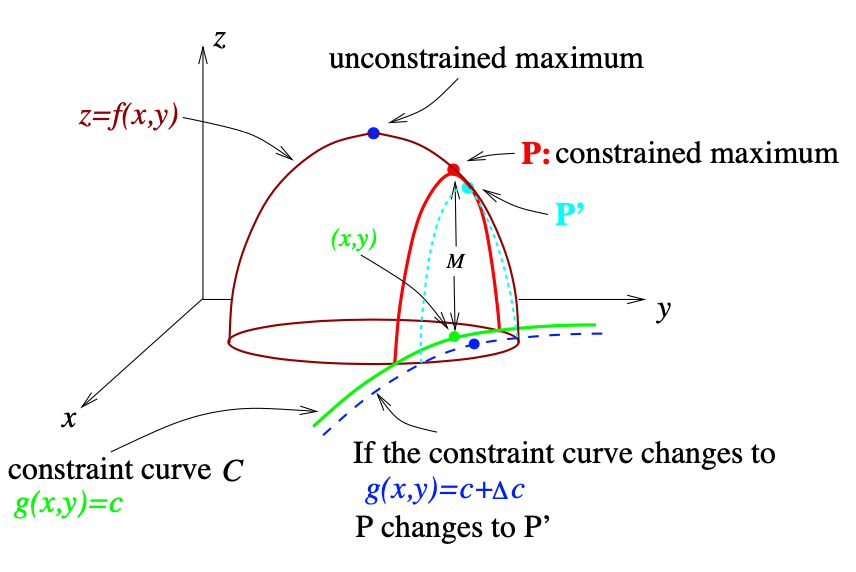
\includegraphics[scale=0.53]{images/Ch13-intepret-lambda.png}
    \end{center}

    \newpage
    {\blue The example below shows the application of $\lambda$.}
    
    \eg Use Lagrangian multiplier to find the maximum and minimum values of the function
    $f(x, y)=4 x^{3}+y^{2}$
    subject to the constraint $2x^{2}+y^{2}=1$.

    If the constraint equation changes to $2 x^{2}+y^{2}=0.9$, 
    estimate how this changes will affect the maximum and minimum values of $f$.

    \sol Let $g(x,y)=2x^2+y^2=1=c$, then for $\nabla f = \lambda \nabla g$, we have
    $(12x^2, 2y)=\lambda (4x, 2y)$, i.e., 
    \begin{align*}
        12x^2 &= \lambda 4x\\
        2y &= \lambda 2y\\
        2x^2+y^2&=1
    \end{align*}
    From the second equation, if $y\ne 0$, then $\lambda = 1$, substitute into the other two equations, 
    we get $\disp (x,y)=(0, \pm 1){\rm \ or\ } \left(\frac{1}{3},\pm \frac{\sqrt{7}}{3}\right)$

    However, if $y=0$, then from third equation, $\disp x=\pm \frac{\sqrt{2}}{2}$, substitute to first eq, 
    we get:
    $$\begin{array}{lll}
        \lambda = \dfrac{3\sqrt{2}}{2} & {\rm when} & x=\dfrac{\sqrt{2}}{2}\\
        \lambda = -\dfrac{3\sqrt{2}}{2} & {\rm when} & x=-\dfrac{\sqrt{2}}{2}
    \end{array}$$

    \begin{center}
        \begin{tabular}{|c|c|c|c|}\hline
            $\lambda$ & $(x,y)$ & $f(x,y)$ & nature \\\hline
            1 & $(0, \pm 1)$ & 1 &  \\\hline
            1 & $\disp \left(\frac{1}{3},\pm \frac{\sqrt{7}}{3}\right)$ & $\disp \frac{25}{27}$ &  \\\hline
            $\disp \frac{3\sqrt{2}}{2}$ & $\disp \left(\frac{\sqrt{2}}{2}, 0\right)$ & $\sqrt{2}$ & max \\\hline
            $\disp -\frac{3\sqrt{2}}{2}$ & $\disp \left(-\frac{\sqrt{2}}{2}, 0\right)$ & $-\sqrt{2}$ & min \\\hline        
        \end{tabular}
    \end{center}
    Since $\disp \frac{dM}{dc}=\lambda$, so $\Delta M\approx \lambda \Delta c$, in this case, $\Delta c=-0.1$, so 
    at min point, 
    $$\Delta M=-\frac{3\sqrt{2}}{2}\cdot (-0.1)=\frac{3\sqrt{2}}{20}\quad {\rm (increase)}$$
    at max point,
    $$\Delta M=\frac{3\sqrt{2}}{2}\cdot (-0.1)=-\frac{3\sqrt{2}}{20}\quad {\rm (decrease)}$$



    \vspace{\fill}
    \begin{center}
        {\it This is the end of Chapter 13.}
    \end{center}
    

\end{spacing}
\end{document}
